% !TEX root = ./paper.tex
\label{sec:content}

In this section, we describe our \tcpls implementation which provides the 
following benefits.
($i$, \textit{Section \ref{sec:prot-multiplexing}}) Applications can use 
parallel 
streams with 
different cryptographic 
contexts and multiplex them over a \tcp connection.
%(mp): TODO reintegrate this whenever the API has substantial text in the body of the paper
%($ii$) An experimental API that wraps \tls and \tcp and enables applications to
%    handle multihoming, multipathing, and various transport layer mechanisms.
%\todo{MP: mettre la ref du workshop et ne pas expliquer}
($ii$) \tcp options can be sent through the secure \tcpls records, improving 
the extensibility of \tcp. We presented this service in a workshop
paper~\cite{rochet2020tcpls} by implementing the \tcp User Timeout option.
%(as described in
   %Section~\ref{sec:background-design})
   %. We demonstrate this possibility by
   %implementing the \tcp User Timeout option%, which is a building block for
   %our Failover protocol
   %.
   %(mp): TODO move this to a section describe secure TCP options, with maybe 
   %the exchange of eBPF code somehow
   % Supporting another \tcp option is only a matter of
   %extending the sender's API and processing the option on the receiver side.
   %\tcpls's internal machinery allows to the server (resp. client) to send any
   %TCP option during (resp. after) the \tls handshake.
($iii$, \textit{Section \ref{sec:prot-migration}}) Applications can trigger 
Connection Migration and enable Failover.
($iv$, \textit{Section \ref{sec:prot-multipath}}) Applications can leverage 
multipath 
capabilities such as stream 
steering %over several \tcp connections 
and bandwidth aggregation.
%\todo{MP: en faire une petite section qui présente l'implémentation, a 
%combiner p-ê avec (ii)}
($v$, \textit{Section \ref{sec:prot-ebpf}}) The server can securely send eBPF 
bytecode to the client 
to upgrade its \tcp congestion control scheme or tune other \tcp 
mechanisms~\cite{brakmo2017tcp,tran2019beyond}. Through these examples,
%hopefully demonstrate how interesting \tcpls's design can be.
we demonstrate that our design enables modern transport services.

%Variable-length options (e.g., eBPF bytecode) can be sent within streams to 
%take advantage of bandwidth aggregation or Failover when these features are 
%enabled.
%($v$) Different connection migration modes: Failover and Application-level
%Connection Migration.
Our prototype is a fork of the \texttt{picotls} \tls 1.3 implementation 
to which we added 9k lines of C code to implement TCPLS.

\subsection{Multiplexing}
\label{sec:prot-multiplexing}

We leverage the \tcpls records and the \tcpls stream cryptographic contexts to 
build our prototype with a zero-copy receive path. When a record is received,
\tcpls first finds the corresponding cryptographic context, i.e. the
corresponding \tcpls stream for which the derived IV leads to a successful
authentication of the tag. This search is limited to the streams attached to 
\tcp connection of the received record. Our prototype tries first the last 
successful \tcpls stream. The receiver only has to find the right cryptographic 
context occasionally depending on the application, i.e. when the sender 
schedules another stream over the \tcp connection.

At this stage, prior to full decryption, the 
\tcpls stream of the record is known. Our prototype can then locate the 
corresponding buffer
to perform full decryption at the expected offset without any extra copy.
Applications can benefit from large contiguous
buffers to perform reads instead of receiving stream data on a per-packet basis,
as often found in QUIC implementations.

%Besides, streams
%are attached to a given \tcp connection (i.e., records of a given stream are 
%all
%sent within the same \tcp connection), leading to a search of the right
%cryptographic context limited to the streams attached to the connection upon
%which the record is received. Note also that the receiver needs to search for
%the right cryptographic context only when the sender writes to another stream 
%(i.e.,
%usually when it has flushed the data of the previous one), meaning that this
%operation is occasional and has negligible impact upon regular usage of the
%protocol

%\fr{I don't want to give the impression that everything works like a charm -- I
%would need 1 more year to have something production ready}
%We stress that all of these features have been tested but this prototype is a
%research-level implementation. The implementation can
%showcase those features but is however not yet ready for production, as many
%bugs likely remain despite our unit tests and integration tests. Portability was
%neither part of our goals, but might be necessary for a production ready \tcpls
%library.

%\subsection{The \tcpls API}
%
%\todo{(mp): How important is this for conext, rather than IETF? I feel like 
%the subsection content is too thin to have any weight}
%
%The API that applications use to interact with a protocol plays an important
%role in leveraging all the protocol features. The most popular
%API to interact with the transport layer remains the BSD socket API. 
%Researchers
%and the IETF have explored new ways to expose a transport
%API~\cite{draft-ietf-taps-arch,hruby2014sockets,rfc6458,schmidt2013socket}.
%Due to space limitations, we provide in appendix~\ref{appendix:api} a simple 
%example of our API workflow,
%which builds upon good practices proposed by the outlined research.

%In this spirit, application-level developers would only be required to
%configure a \tcpls context and register function callbacks.
%We design \tcpls such
%that the application-level developers can ignore any notion of Network IPC as
%defined by, for example, the POSIX API, the Berkeley socket API or Winsock,
%facilitating application-level development by offering a more concrete
%session-level interface based on asynchronous network events.
%The overall idea is to offer to application developers the opportunity to tune
%the transport protocol for a better usage of the network from their own
%application protocol, which might depend on its distinguishing
%features.
%\todo{we need to explain the mpjoin}


%Note, those features are not stable yet, and many bugs remain to be fixed.

\subsection{Failover}
\label{sec:prot-migration}

%\textbf{Failover}.
We leverage the \tcpls records to securely exchange the \tcp User Timeout option.
This option enables endpoints to detect blackholed and failed \tcp connections
after a given time threshold. We use this as one trigger of the Failover. The 
sender configures this time threshold at the receiver side by sending this \tcp 
option in a \tcpls record. The receiver can then notice when it stops receiving 
data and trigger the Failover.
Receiving a \tcp \texttt{RST} or \texttt{FIN} over a \tcp connection for which
\tcpls streams are attached does also trigger the Failover.

The stream-level acknowledgments required for the Failover to detect the lost
\tcpls records can be enabled at the start of a \tcpls session. The default
policy is to acknowledge every 16 received records, or when a
stream has processed 
%more than $249600$ 
%\todo{Maybe explain the number?}
a given amount of 
bytes since the last acknowledgment. 

Our prototype handles failover over IPv4 and IPv6 \tcp connections, and by default, chooses different source and destination addresses than the failed \tcp connection if possible.

Application running on more constrained devices can choose to disable Failover
to gain in performance. They can also enable Failover during a \tcpls session 
by sending a message on the secure channel. 
We evaluate the performance impact of Failover in 
Section~\ref{sec:eval_failover}

%\textbf{Application Connection Migration}.
%\todo{Is there something to write implementation-wise?}

\subsection{Multipath}
\label{sec:prot-multipath}

\textbf{Stream steering}.
\tcpls exposes the \tcp connections it manages to the application. This allows 
the application to directly distribute the \tcpls streams over the \tcp 
connections at any point of the \tcpls session. A simple distribution is to 
move all \tcpls streams from one connection to another, as performed during 
Application-triggered Connection Migration. Our prototype enables these 
operations in a few API calls. More complex stream attachment policies can be 
implemented by the application to meet its requirements.
%The application, using our \tcpls API can create, attach and steer data within
%any \tcp connection previously created using  \texttt{tcpls\_connect()} and 
%joined using
%\texttt{tcpls\_handshake()}. Properties over the streams can be negotiated, 
%such as the
%failover mode (global to all streams) or \textit{Coupled Streams}, that let the
%application uses the same interface \texttt{tcpls\_send()}  and 
%\texttt{tcpls\_receive()}
%independently of the negotiated stream features. As a matter of example, Stream
%steering and \textit{Coupled Streams} can offer the application to steer a
%connection migration (so called Application Connection Migration in
%section~\ref{sec:transport-services}) in four API calls (i.e., creating a \tcp
%connection, joining the \tcpls session, creating a stream and closing previous
%streams).

\textbf{Bandwidth Aggregation}.
The application can create and join several \tcp connections to
the same \tcpls session. When coupled streams are attached to
different \tcp connections, \tcpls adds a sequence number encrypted in the \tls 
record payload. It is used to reorder the received records 
after decryption. Our prototype only supports coupling all streams together.
%, but
%we envision for the \tcpls protocol to have streams potentially detached from
%the global orderings. 
%For example, a HTTP application may want to use an
%aggregation mode for 2 streams over 2 \tcp connections downloading a video
%content for the video playback engine, but the other streams used by the HTTP
%client do not necessarily need to be part of the multipath bandwidth 
%aggregation.
%Such a feature may be implemented through a negotiation of the aggregation 
%mode.
The sending application implements the scheduling coupled streams over the 
different \tcpls connections.
Our implementation currently includes a round-robin scheduler on the receiver
side. We expect to
support other schedulers in the future and allow the application to select its 
preferred scheduler through the API, or even send it as eBPF bytecode over the 
session. The more \tcpls receives records in order, the more it can deliver 
them in a zero-copy fashion to the application. When a record is received 
out-of-sequence, its content is pushed on an efficient reordering heap. %in 
%$O(log(n))$ for $n$ elements in the heap. Checking the minimum sequence number 
%in the heap is in $\Theta(1)$ and retrieving is in $O(log(n))$. 
The performance of our multipath bandwidth aggregation is evaluated in
Sec.~\ref{sec:bwaggr}.

%\subsubsection{Failover}\label{failover}
%Failover is a binary mode (on/off) that is fully internal to \tcpls.
%Once activated, \tcpls exchanges acknowledgments for records received on each
%stream. These acknowldgments are stream-based and configurable. The default
%acknowledgment policy is to acknowledge every 16 received records, or when a
%stream has processed more than $249,600$ bytes since the last acknowledgment.
%When a \tcp connection conveying \tcpls streams suffers from a network outage (e.g., a \rst is received or the connection becomes idle for too long), we move the stream to a new \tcp connection, retransmit the unacked records, and resume the transfer. Our prototype handles failover over IPv4 and IPv6 \tcp connections, and by default, chooses different source and destination addresses than the failed \tcp connection if some are available.
%%Failover might be negotiated by both party, or
%%enabled by default by both party.
%Depending on the application type, Failover might be enabled or not by 
%default. It is also possible to activate Failover during a \tcpls session by 
%sending a message on the secure channel. We evaluate the performance of 
%Failover in Section~\ref{sec:eval_failover}

%\subsubsection{Application-level Connection Migration}
%\label{sec:connmigr}


%When an application feels right to migrate its connection, it
%can follow those simple steps: activating the multipath aggregation
%mode, then making a \tcpls join handshake on the new path. Then, opening a new stream
%and attaching it to the new \tcp connection, and closing the initial
%stream would make the data transfert enter in a temporary two-paths aggregated mode in
%which the other peer's first path flushes its data if any, and then gracefully close the \tcp
%connection achieving a smooth migration. In practice, such a migration would
%achieve better goodput than a QUIC single-path migration design in which the
%data path is temporally broken and then recovered. In our design, the
%application can make such a migration in 5 API calls.

%\subsection{TCP Options and Kernel extensibility}

\subsection{eBPF code remote attachment}
\label{sec:prot-ebpf}

Recent work on restructuring congestion control has proposed a generic 
architecture for congestion controllers~\cite{narayan2018restructuring}.
Linux kernel developers have relied on eBPF to make the Linux TCP/IP 
stack easier to extend~\cite{brakmo2017tcp,tran2020beyond}. Since Linux kernel 
version 5.6, an application can attach congestion control schemes 
entirely implemented in eBPF. A broader approach was proposed for \quic in 
Pluginizing \quic~\cite{de2019pluginizing}. 
%We leverage these new eBPF capabilities to demonstrate the feasibility of 
%injecting a new congestion control scheme during a \tcpls session.

Our \tcpls prototype enables the server %to use \tcpls streams 
to attach a new eBPF congestion controller to the client over the \tcpls 
session. The type of eBPF code 
that can be attached could be easily extended to other points of the TCP 
execution path.
The eBPF code is conveyed securely in a dedicated \tcpls record. When 
the code is larger than a single \tls record, it can be chunked in several 
records and sent using a \tcpls stream cryptographic context. This service 
illustrates how the flexibility of \tcpls record and streams can be leveraged 
to implement novel transport mechanisms.

%The \tcpls streams enable new use cases. A \tcpls application can
%create and use different streams to carry data. However, since these streams
%are generic, they can also be used by the \tcpls implementation itself to
%exchange control information. To demonstrate the versatility of these control
%streams, we extended \tcpls to enable a server to push a different congestion
%control scheme to a specific client over an existing \tcpls session. 
\subsection{\tcpls Session Establishment}

Our prototype is fully compatible with \tls 1.3 0-RTT session resumption
and \tcp Fast Open option (TFO)~\cite{radhakrishnan2011tcp}. By combining them,
the \tcpls handshake can be sent together with the \tcp \texttt{SYN} starting 
the three-way handshake. This provides a low-latency and secure connection establishment.
It is not enabled by default in \tcpls, as TFO trades off some privacy~\cite{sy2020enhanced}.
More advanced techniques such as \tcp Fast Open Privacy~\cite{sy2020enhanced} 
could be
integrated into \tcpls to solve this issue.

\subsection{\tcpls API}
\label{sec-api}

The API used by applications to interact with a protocol plays an important
role in leveraging all the protocol features. The most popular
API to interact with the transport layer is the BSD socket API. 
But researchers and the IETF have explored other ways to expose a transport
API~\cite{draft-ietf-taps-arch,hruby2014sockets,rfc6458,schmidt2013socket}.

The \tcpls API builds upon good practices proposed by the outlined research.
In this spirit, application-level developers are only required to
configure a \tcpls context and register function callbacks.
We design the \tcpls API such
that application-level developers can ignore any notion of inter-process 
communication, e.g. as defined by the POSIX API, the Berkeley socket API or 
Winsock, facilitating application-level development by offering a more concrete
session-level interface based on asynchronous network events.
The \tcpls API offers the opportunity to tune
the transport protocol to application developers. They can then make the best 
choices for their applications.
% for a better usage of the 
%network from their own application protocol, which might depend on its 
%distinguishing
%features.

As an example illustrating the flexibility of the \tcpls API, we consider a 
simple use case inspired by Happy Eyeballs~\cite{rfc8305}. This technique is
used by web browsers when interacting with dual-stack servers. They
start parallel \tcp connections using IPv4 and IPv6 and then choose the
one that offers the lowest latency. This avoids problems when one type of 
address is not supported on a network path but not the other, or when one 
results in lower latency~\cite{bajpai2019longitudinal}.

\begin{figure}[!t]
	\resizebox{0.49\textwidth}{!}{%
		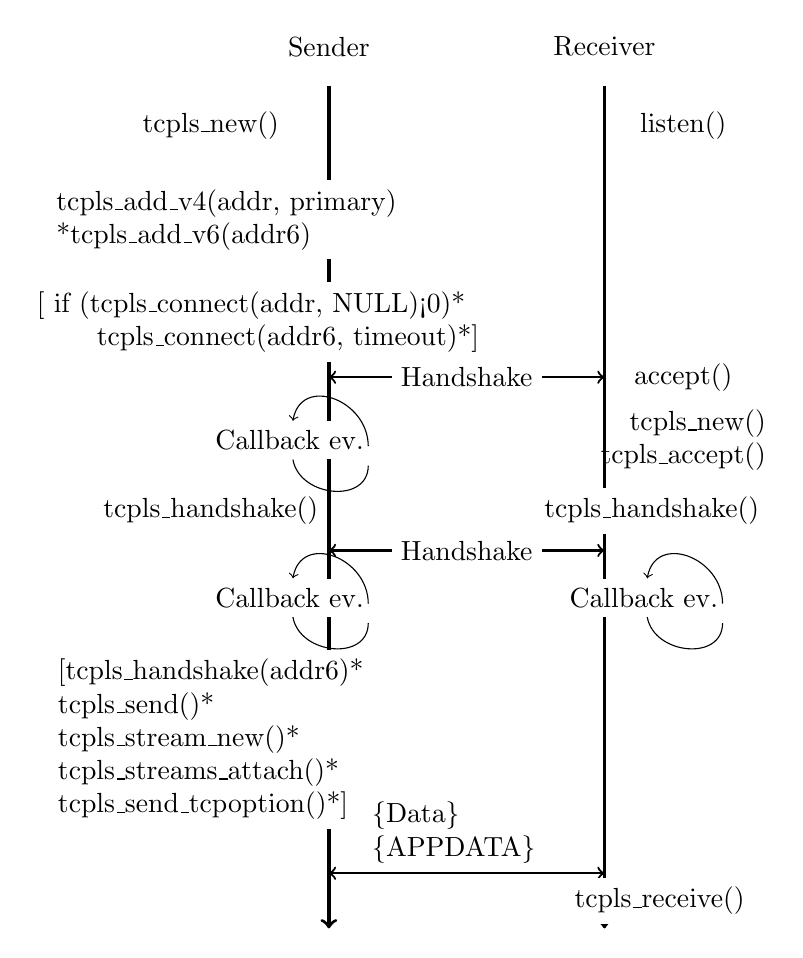
\begin{tikzpicture}
			\colorlet{lightgray}{black!20}
			\tikzstyle{arrow} = [thick,->,>=stealth]
			\tikzset{state/.style={rectangle, dashed, draw, fill=white} }
			\node[black, fill=white] at (0.5,10) {Sender};
			\node[black, fill=white] at (4,10) {Receiver};
			\draw[very thick,->] (0.5,9.5) -- (0.5,-1.2);
			\draw[very thick,->] (4,9.5) -- (4,-1.2);
			\node at (-1,9) {tcpls\_new()};
			\node at (5, 9) {listen()};
			\node[align=left, fill=white] at (-0.8,7.8) {tcpls\_add\_v4(addr,
				primary)\\*tcpls\_add\_v6(addr6)};
			\node[fill=white, align=left] at (-0.4,6.5) {[ if 
			(tcpls\_connect(addr,
				NULL)<0)*\\
				\indent~~tcpls\_connect(addr6, timeout)*]};
			\draw[black, thick, <->] (0.5,5.8) -- (4,5.8) node [midway, 
			fill=white] {\tcp Handshake};
			\node[fill=white] at (0,5) (Callback) {Callback ev.};
			\node at (1,4.8) (here) {};
			\draw [->] (Callback) to[out=-80, in=-90,looseness=1.3] (here)
			to[out=90,in=80,looseness=1.5] (Callback);
			\node at (5, 5.8) {accept()};
			\node[align=right] at (5, 5) {tcpls\_new()\\tcpls\_accept()};
			\node at (-1,4.1) {tcpls\_handshake()};
			\node[fill=white] at (4.6,4.1) {tcpls\_handshake()};
			\draw[black, thick, <->] (0.5,3.6) -- (4,3.6) node [midway, 
			fill=white] {\tcpls Handshake};
			\node[fill=white] at (0,3) (CB2) {Callback ev.};
			\node at (1,2.8) (here2) {};
			\draw [->] (CB2) to[out=-80, in=-90,looseness=1.3] (here2)
			to[out=90,in=80,looseness=1.5] (CB2);
			\node[fill=white] at (4.5,3) (CB3) {Callback ev.};
			\node at (5.5,2.8) (here3) {};
			\draw [->] (CB3) to[out=-80, in=-90,looseness=1.3] (here3)
			to[out=90,in=80,looseness=1.5] (CB3);
			\node[fill=white, align=left] at (-1, 1.2)
			{[tcpls\_handshake(addr6)*\\tcpls\_send()*\\tcpls\_stream\_new()*\\tcpls\_streams\_attach()*\\tcpls\_send\_tcpoption()*]};
			\draw[black, thick, <->] (0.5,-0.5) -- (4,-0.5) node [midway, 
			fill=white,
			above, text width=2.4cm]
			{\{\tcpls Data\} \{APPDATA\}};
			\node[fill=white] at (4.7,-0.85) {tcpls\_receive()};
		\end{tikzpicture}
	}
	\caption{API Workflow example. * means optional call, [ ] means optional 
	call flow, and \{ \} means encrypted.}
	\label{fig:api}
\end{figure}

Figure~\ref{fig:api} shows an example of our current API workflow. The API can
handle explicit multipath techniques such as Happy Eyeball by chaining
\texttt{tcpls\_connect()} with an appropriate timeout of 50ms, as shown in the
Figure. \tcpls lets the application explicitly choose the pairs of addresses 
between which a TCP connection should be established by
calling several times \texttt{tcpls\_connect(src, dest, timeout)}. The
application may configure callbacks to connection events that occur within
\tcpls, such as connection establishments, stream attachments, multipath
joins, the receipt of a \tcp option to tune \tcp. 

%When streams are attached to multiple \tcp connections, the application may 
%configure various \tcpls behaviours. Among them, we support HOL-blocking 
%avoidance,
%aggregation of bandwidth with multipathing, connection failover, and connection
%migration. Note that, HOL-blocking avoidance is incompatible with
%aggregating bandwidth using multipathing (the application cannot enable both
%features at the same time).


%One notable feature of \quic is its ability to establish a secure connection within one round-trip-time with a new server. For subsequent connections with the same server, \quic can even include data during the handshake.

%\tls 1.3 also includes a fast handshake for subsequent connections. When used with \tcp Fast Open (TFO)~\cite{radhakrishnan2011tcp}, the \tls handshake can be sent together with \tcp's three way handshake. However, TFO suffers from privacy issues~\cite{sy2020enhanced}. For this reason, we did not enable it by default in \tcpls. We could revise this decision if a solution similar to \tcp
%FOP~\cite{sy2020enhanced} is included in mainline TCP implementations.


%One argument for QUIC's usage on the web was its first 1-rtt secure connection.
%Compared to TLS/TCP, QUIC has only one handshake and can then proceed with the
%application data. $TLS/TCP$ has two: First, the \tcp three-way handshake, and
%then the \tls handshake.

%\tcpls can use \tcp's TFO~\cite{radhakrishnan2011tcp}
%and send the \texttt{ClientHello} message within the \tcp SYN's payload,
%achieving the same roundtrips than QUIC. However, TFO suffers from privacy
%issues~\cite{sy2020enhanced}, thus we did not enable it by default. In the
%future, we may expect to revise our choice if a solution similar to \tcp
%FOP~\cite{sy2020enhanced} gets implemented in the Linux kernel.
